\subsection{Scenario Definition}
The simplified transition scenario modeled was from the current once-through
Light Water Reactor (LWR) fuel cycle, to a fleet of Sodium Fast Reactors (SFR)
with 100\% recycle of spent fuel.  The simulation starts in January 2014 and
lasts until transition to 100\% SFRs is complete. The nuclear installed
capacity is constant (100GWe).

The transition is driven by the criteria that when sufficient separated
material is present, an LWR ($1000$MWe) should be decommissioned and replaced
with three ($333.\bar{3}$) SFRs.

A summary of the material flows in the simulation can be found in Figure 
\ref{fig:cycic_img}. 

\begin{figure}[htpb!]
\begin{center}
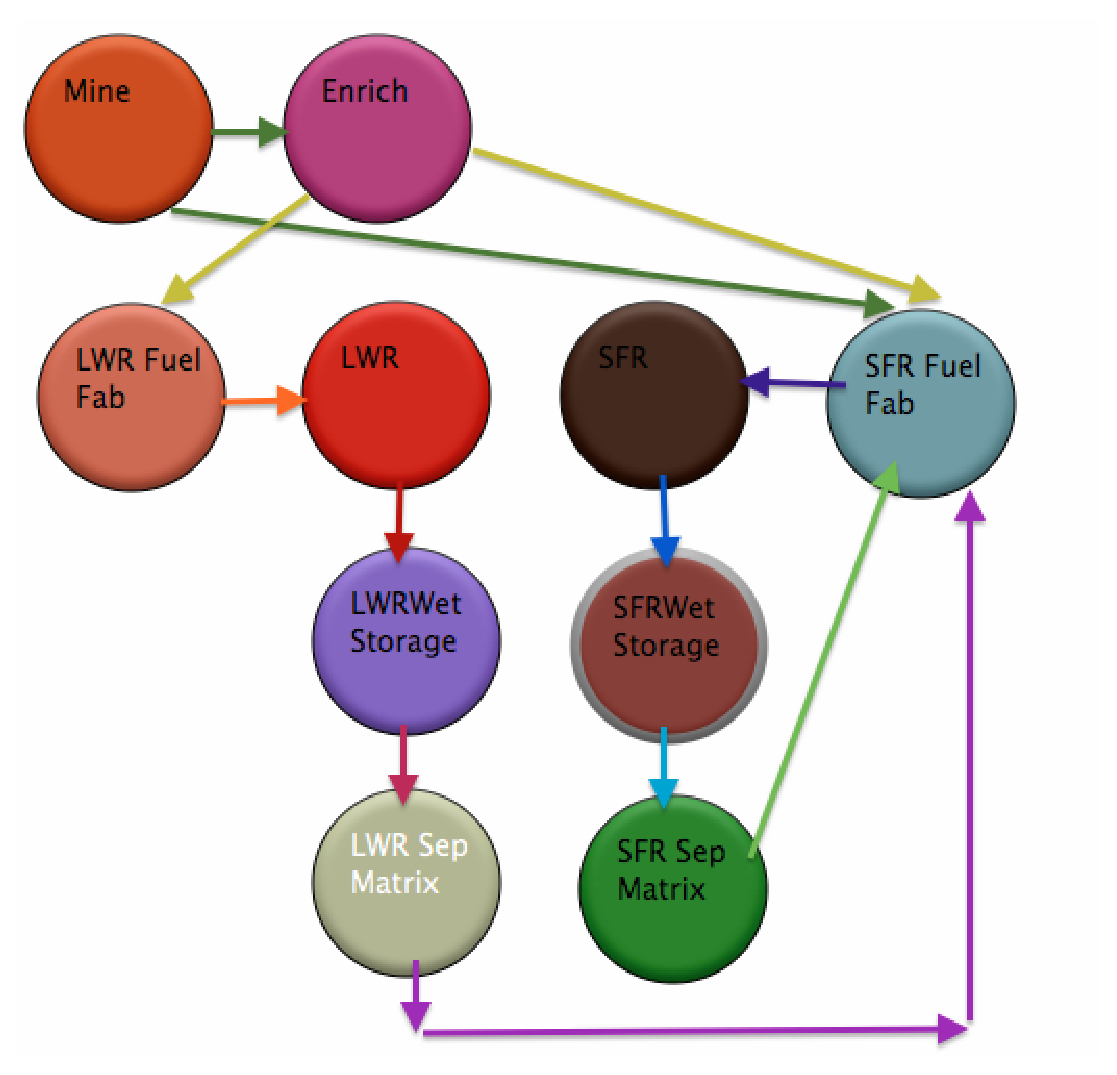
\includegraphics[width=0.45\textwidth]{cycic_img.eps}
\end{center}
\caption{The basic material flow paths for this simulation. This image was 
generated by Cycic, the input controller for \Cyclus 
\cite{flanagan_input_2013}.}
\label{fig:cycic_img}
\end{figure}

\subsubsection{Deployment Regions and Institutions}

In order to facilitate a deployment profile for the LWR to SFR transition, an 
existing Cycamore model was used. The GrowthRegion model maintains a 
power generation profile specified by the user. It does this by deploying or 
decommissioning reactors when necessary to maintain the specified growth 
profile.  

In this case, a constant 100GWe ``growth'' is maintained in the simulation. 
This region encapsulates all of the facilities in this simulation. 
When sufficient material is available to support a new set of three SFRs, an 
LWR is decommissioned. When power generating capacity is lost due to an LWR 
(1000MWe) decommissioning, the GrowthRegion deploys sufficient SFR capacity 
(three 333.3MWe SFRs) to replace it. 

An entity that decommissions LWRs based on material availability was not 
present in the default models, however. To support this ability, an extension 
model was implemented as a ``Decommissioning Facility.'' That model is 
addressed in Section \ref{sec:decomminst}.

\subsubsection{Commodities}

%\begin{multicols}{1}
\begin{table}[htbp!]
\centering
\begin{tabular}{|l|l|l|}
\hline
Commodity  &     Offered By  &    Requested By \\
\hline
Natural  U & Mine & Enrichment \\ 
LEU & Enrichment & LWRFuelFab \\ 
Depleted U & Enrichment & SFRFuelFab \\ 
fresh LWR fuel & LWRFuelFab & LWR \\ 
fresh SFR fuel & SFRFuelFab & SFR \\ 
LWR UNF & LWR & LWRWetStorage \\ 
SFR UNF & SFR & SFRWetStorage \\ 
cool LWR UNF & LWRWetStorage & LWRSeparation \\ 
cool SFR UNF & SFRWetStorage & SFRSeparation \\ 
separated LWR U & LWRSeparation & SFRFuelFab \\ 
separated LWR TRU & LWRSeparation & SFRFuelFab \\ 
separated SFR U & SFRSeparation & SFRFuelFab \\ 
separated SFR TRU & SFRSeparation & SFRFuelFab \\ 
\hline
\end{tabular}
\caption{Commodity flow in the transition simulation}
\label{tab:commods}
\end{table}
%\end{multicols}
Note that the exact compositions of U and TRU were not given. These will be
approximated by representative isotopes in the \Cyclus definition.

\subsubsection{Facility Implementations}

\begin{table}[htbp!]
\centering
\begin{tabular}{|l|l|r|}
\hline
\textbf{Facility Type} &\textbf{Agent} & \textbf{Key Parameters}\\
\hline
Mine & SourceFacility & Capacity\\
\hline
Enrichment & EnrichmentFacility & feed enrchment\% \\
& & tails enrichment\% \\
& & Process time \\
\hline
LWRFuelFab & StreamBlender & Process time\\
& & Fissile Source\\
\hline
SFRFuelFab & StreamBlender  & Process time\\
& & Fissile Sources\\
& & Fertile Sources\\
\hline
LWR & BatchReactor & Installed Capacity \\
& & Capacity Factor \\
& & Batches per core \\ 
& & Cycle length\\
& & Fresh Fuel Comp. \\
& & Spent Fuel Comp. \\
\hline
SFR & BatchReactor & Installed Capacity\\
& & Capacity Factor \\
& & Batches per core \\ 
& & Cycle length\\
& & Fresh Fuel Comp. \\
& & Spent Fuel Comp. \\
\hline
LWRWetStorage & CommodConverter & Process time\\
\hline
SFRWetStorage & CommodConverter & Process time\\
\hline
LWRSeparation & SeparationMatrix & Capacity\\
& & Process Time\\
& & Efficiency Matrix\\
\hline
SFRSeparation & SeparationMatrix & Capacity\\
& & Process Time\\
& & Efficiency Matrix\\
\hline
HLW Repository & SinkFacility & Capacity \\
\hline
\end{tabular}
\caption{Facilities and their implementations with key parameters.}
\label{tab:facimpl}
\end{table}
\FloatBarrier

\subsubsection{Desired Outputs}

The desired outputs of this simulation include deployment metrics such as the 
year during which the transition becomes complete and capacity profiles over 
time. These profiles should demonstrate that there were no potential generating 
shortages. Additionally, material metrics such as separated surplus PU or TRU 
profiles, LWR used fuel reprocessing rate (t/yr), SFR used fuel reprocessing 
rate (t/yr),  LWR used fuel mass in storage (t), and SFR used fuel mass in 
storage (t).
